%%%%%%%%%%%%%%%%%%%%%%%%%%%%%%%%%%%%%%%%%%%%%%%%%%%%%%%%%%%%%%%%%%%%%%
% LaTeX Example: Project Report
%
% Source: http://www.howtotex.com
%
% Feel free to distribute this example, but please keep the referral
% to howtotex.com
% Date: March 2011 
% 
%%%%%%%%%%%%%%%%%%%%%%%%%%%%%%%%%%%%%%%%%%%%%%%%%%%%%%%%%%%%%%%%%%%%%%
% How to use writeLaTeX: 
%
% You edit the source code here on the left, and the preview on the
% right shows you the result within a few seconds.
%
% Bookmark this page and share the URL with your co-authors. They can
% edit at the same time!
%
% You can upload figures, bibliographies, custom classes and
% styles using the files menu.
%
% If you're new to LaTeX, the wikibook is a great place to start:
% http://en.wikibooks.org/wiki/LaTeX
%
%%%%%%%%%%%%%%%%%%%%%%%%%%%%%%%%%%%%%%%%%%%%%%%%%%%%%%%%%%%%%%%%%%%%%%
% Edit the title below to update the display in My Documents
%\title{Project Report}
%
%%% Preamble
\documentclass[paper=a4, fontsize=11pt]{scrartcl}
\usepackage[T1]{fontenc}
\usepackage{fourier}

\usepackage[english]{babel}															% English language/hyphenation
\usepackage[protrusion=true,expansion=true]{microtype}	
\usepackage{amsmath,amsfonts,amsthm} % Math packages
\usepackage[pdftex]{graphicx}	
\usepackage{url}
\usepackage[]{algorithm2e}
\usepackage{float}

%%% Custom sectioning
\usepackage{sectsty}
\allsectionsfont{\centering \normalfont\scshape}


%%% Custom headers/footers (fancyhdr package)
\usepackage{fancyhdr}
\pagestyle{fancyplain}
\fancyhead{}											% No page header
\fancyfoot[L]{}											% Empty 
\fancyfoot[C]{}											% Empty
\fancyfoot[R]{\thepage}									% Pagenumbering
\renewcommand{\headrulewidth}{0pt}			% Remove header underlines
\renewcommand{\footrulewidth}{0pt}				% Remove footer underlines
\setlength{\headheight}{13.6pt}


%%% Equation and float numbering
\numberwithin{equation}{section}		% Equationnumbering: section.eq#
\numberwithin{figure}{section}			% Figurenumbering: section.fig#
\numberwithin{table}{section}				% Tablenumbering: section.tab#


%%% Maketitle metadata
\newcommand{\horrule}[1]{\rule{\linewidth}{#1}} 	% Horizontal rule

\title{
		%\vspace{-1in} 	
		\usefont{OT1}{bch}{b}{n}
		\normalfont \normalsize \textsc{Computational Geometry} \\ [25pt]
		\horrule{0.5pt} \\[0.4cm]
		\huge Interactive KD-Tree Implementation \\
		\horrule{2pt} \\[0.5cm]
}
\author{
		\normalfont 								\normalsize
        Gautam Kumar  \\[-3pt]		\normalsize
        Vitaly Sergeyev \\[-3pt]    \normalsize
        \today
}
\date{}


%%% Begin document
\begin{document}
\maketitle
\section{Abstract}
A KD-Tree is a popular binary-tree datastructure used in many applications such
as range-search and nearest-neighbor search. The algorithm to build a kd-tree
partitions k dimension input space based on the median points in the spacial
frame. This type of data-structure makes searching for points in space an aver-
age O(logn) algorithm. While a query with an axis-parallel rectangle in a KD-Tree storing n points can be performed in O( $(n)^{1 - \frac{1}{d}}$ + k) time, where k is the number of reported points and d is dimension.

\section{Project Overview}
We have implemented an interactive 2D KD-Tree application. The user can click a set
of points in a 2D input space or program can read the point set from the input file, after which the application visualize the kd-tree partitions and the tree itself. The user can also draw a bounding box on the screen to capture points in the plane or program can randomly draw the bounding box. Performance time is a metric of input size as well time. We have also implemented methods to generate a large, uniformly distributed set of points for input to the KD-Tree implementation. On top of that, we have analyzed and build a plot for analyzing the performance of the KD-Tree range search vs the brute force approach. We have the report on the N values that show a significant improvement in performance over the brute-force approach.

\section{Implementation Details}
We have mainly used following classes.
\begin{enumerate}
\item \textbf{Point:} It represents a two dimensional point in the 2-D space. It has x and y co-ordinates as attributes. It also consist the methods to do basic operations on point set. In our implementation a point object requires 16 bytes of memory. It has been implemented in \textbf{Point2D.java}.
\item \textbf{RectHV:} It represents a rectangle in 2-D space. A rectangle has been represented by lower leftmost point and upper rightmost point. It also has method to check whether two rectangles intersect each other or not. In our implementation a RectHV object requires 32 bytes of memory. It has been implemented in \textbf{RectHV.java}.
\item \textbf{KdTree:} It represents the KD-Tree in 2-D space. Node structure of KD-Tree consists of point associated with that node, rectangle represented by that node, and left, right children of that node. It also provides methods for various operations (insert, search, draw) on KD-Tree. In our implementation a Node object requires 64 bytes of memory. It has been implemented in \textbf{KdTree.java}.
\item \textbf{KdTreeVisualizer:} It provides the graphical view of KD-Tree as well as execution of building of KD-Tree. It has been implemented in \textbf{KdTreeVisualizer.java}.

\item \textbf{RangeSearchVisualizer:} It provides the graphical view of range search execution on point set. It uses KD-Tree search as well brute force search method. It has been implemented in \textbf{RangeSearchVisualizer.java}.
\end{enumerate}
\pagebreak
We have implemented following algorithms.\\
\begin{itemize}
\item BUILDKDTREE(P, depth)

\begin{algorithm}[H]
 \KwData{A set of points \textit{P} and the current depth \textit{depth}}
 \KwResult{The root of a kd-tree storing \textit{P} }
 initialization\;
  \eIf{P contains only one point}{
   return a leaf storing this point\;
   }{
   \eIf{depth is even}{
Split P into two subsets with a vertical line L through the
median x-coordinate of the points in P. Let P1 be the set of
points to the left of L or on , and let P2 be the set of points
to the right of L.\;
   }
   {Split P into two subsets with a horizontal line L through
the median y-coordinate of the points in P. Let P1 be the
set of points below or on L, and let P2 be the set of points
above L.\;
}
}
$v_{left} \leftarrow$ BUILDKDTREE(P1, depth+1)\;
$v_{right} \leftarrow$ BUILDKDTREE(P2, depth+1)\;
Create a node $v$ storing L, make $v_{left}$ the left child of $v$, and make $v_{right}$ the right child of $v$\;
return $v$\;
% \caption{How to write algorithms}
\end{algorithm}
\textbf{Analysis:} A kd-tree for a set of n points uses O(n) storage and can be constructed in O(n log n) time.


\pagebreak
\item SEARCHKDTREE($v$, R)

\begin{algorithm}[H]
 \KwData{The root of (a subtree of) a kd-tree, and a range R.}
 \KwResult{All points at leaves below ν that lie in the range. }
 initialization\;
  \eIf{if $v$ is leaf}
   {
      Report the point stored at $v$ if it lies in R.\;
   }
   {
      \eIf{region($lc(v)$) is fully contained in R}
      {
        REPORTSUBTREE(lc(ν))\;
      }
      {
	      \eIf{region($lc(v)$) intersects R}
	      {
	        SEARCHKDTREE($lc(v)$, R)\;
	      }	
	      {

	      }
      }
      \eIf{region($rc(v)$) is fully contained in R}
      {
        REPORTSUBTREE(rc(ν))\;
      }
      {
	      \eIf{region($rc(v)$) intersects R}
	      {
	        SEARCHKDTREE($rc(v)$, R)\;
	      }	
	      {

	      }
      }
   }
\end{algorithm}
\end{itemize}
\textbf{Analysis:} A query with an axis-parallel rectangle in a kd-tree storing n points can be performed in $O(\sqrt[2]{n} + k)$ time, where k is the number of reported points.



\pagebreak
\section{How to use}
Goto the directory which has the source files.\\
Type make
\begin{itemize}
\item Build KD-Tree: Type java KdTreeVisualizer 
  It will popup a window, you can click the point and hit enter.
  It will show you KD-Tree, now you can draw a rectangle on it.
  and it will show you the point inside the rectangle in blue color.
  \item Build Range-Search: Type java RangeSearchVisualizer <filename> (Your file name should conatin point in 2-D space between 0 to 1). It will popup a window with points plotted on it. you can draw rectangle over it and color those points which are inside the rectangle. The blue color represents the points discovered by KD-Tree search while red color represents the points discovered by brute search. In the background terminal you can also see the time take by both methods. 
  
\end{itemize}

\section{Experiment}
We compared the KD tree implementation method with brute force method for various values of point set. We uniformly randomly generated the point sets between 0-1 and query rectangle of size 0-0.1. We ploted the graph (figure 4.1) of time taken by both methods for axis-aligned query.

\begin{figure}[H]
\centering
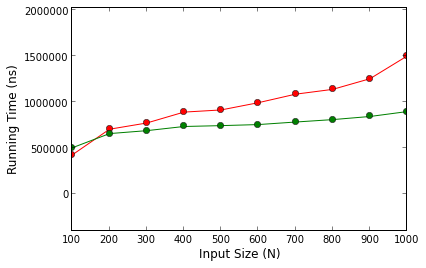
\includegraphics[width=0.47\textwidth]{index.png}
\caption{Red curve for brute force, green curve for KD-Tree}
\end{figure}
 


\begin{thebibliography}{9}

\bibitem{lamport94}
Computational Geometry: Algorithms and Applications.
\bibitem{}
https://www.cs.princeton.edu/courses/archive/fall12/cos226/assignments/kdtree.html
\end{thebibliography}
%%% End document
\end{document}